\documentclass[12pt]{beamer}
\usepackage[utf8]{inputenc}
\usepackage[german]{babel}
\usepackage{amsmath}
\usepackage{graphicx}
\usetheme{default}
\setbeamertemplate{footline}[frame number]
\begin{document}
	\author{Moritz Berger, Tim Herbermann,\\ Gerald Kolter, Sebastian Siebert}
	\title{Akustik}
	\subtitle{Grundpraktikum Teil I}
	%\logo{}
	%\institute{}
	%\date{}
	%\subject{}
	%\setbeamercovered{transparent}
	\setbeamertemplate{navigation symbols}{}
	\frame[plain]{\maketitle}
	

	\begin{frame}
		\frametitle{Schall in Gasen - Ausbreitung}
		\begin{itemize}
		\item Schalldruck  $p(x, t) = p_0 cos(kt + \omega t)$
		\item Wellenzahl $k = 2\pi / \lambda$ und Kreisfrequenz $\omega = 2\pi f$
		\item Schallausbreitung mit $v = \frac{\Delta s}{\Delta t} = \lambda f$
		\end{itemize}
		\begin{itemize}
		\item $v_{Schall} = v_0 \sqrt{T/T_0} \text{\qquad mit \qquad} v_0 = \sqrt{\frac{R\cdot\kappa}{M_{mol}}T_0}$
		\end{itemize}
		
	\end{frame}
	
	\begin{frame}
		\frametitle{Schall in Gasen - stehende Wellen}
		\begin{itemize}
		\item $\hat{p}(x) = \rho v \frac{u_L}{\sqrt{2}} \cos kx/\sin kL$\\ [0.6cm]
		\item Druckknoten: $\Delta x = \lambda / 2$\\ [0.2cm]
		\item $x_n = n \lambda/2 - \lambda/4$\\ [0.45cm]
		\item Resonanzen: $f_n = n v/2L$
		\end{itemize}
		
	\end{frame}

	\begin{frame}
		\frametitle{Kalibration Potentiometer}
		\begin{center}
			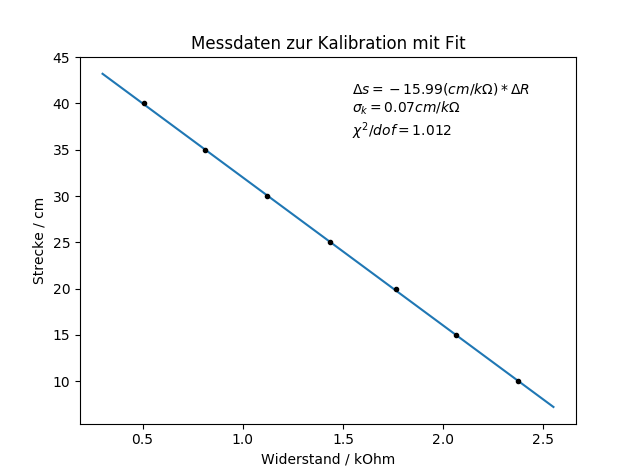
\includegraphics[width=0.6\linewidth]{kalibration_poti_fit}
			
			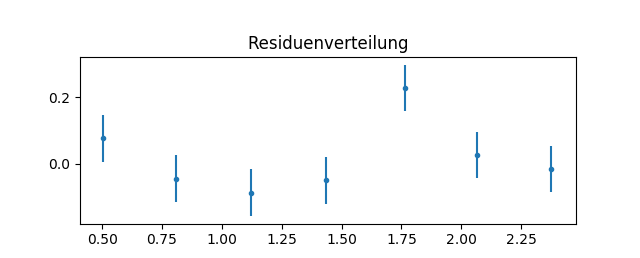
\includegraphics[width=0.6\linewidth]{residuen_kalibration}
		\end{center}
		
	\end{frame}

	
	\begin{frame}
		\frametitle{Laufzeitmessung \qquad Versuchsaufbau}
		\begin{center}
			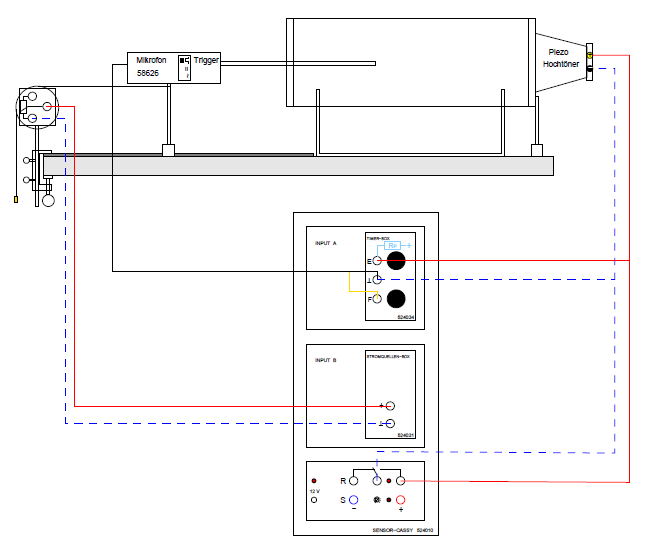
\includegraphics[width=0.6\linewidth]{aufbau_laufzeitmessung}
		\end{center}
			CASSY Kanal A Laufzeit Dta1 E $\rightarrow$F, 2ms, Flanken invertiert \\
			Relais frac(time) \textless 0.1\\
			Messparameter  automatisch Intervall 1s \\
			neue Messreihe anhängen

	\end{frame}

	\begin{frame}
		\frametitle{Laufzeitmessung \qquad Rohdaten}
		\begin{center}
			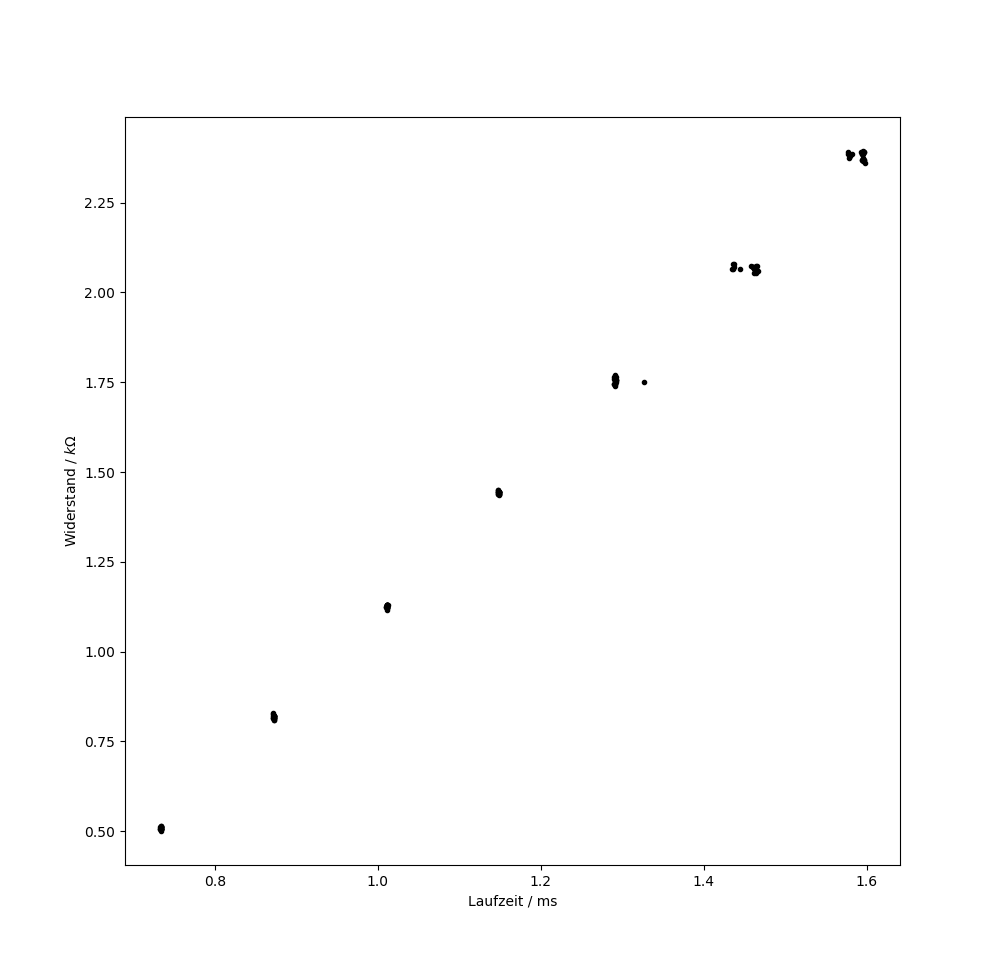
\includegraphics[width=0.75\linewidth]{rohdaten_laufzeit}
		\end{center}
	\end{frame}

	\begin{frame}
		\frametitle{Laufzeitmessung \qquad Auswertung I}
		\begin{center}
			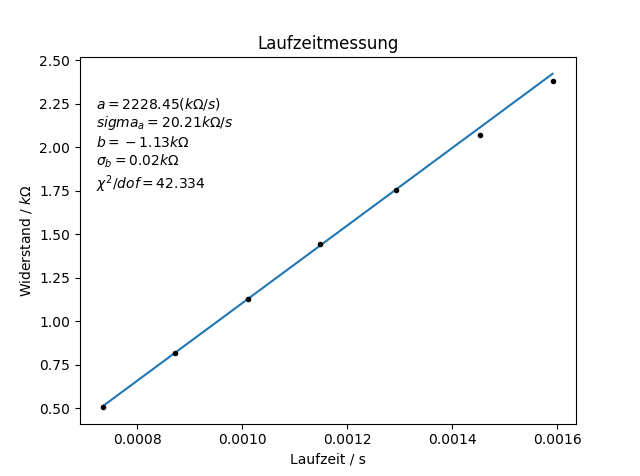
\includegraphics[width=0.6\linewidth]{fit_laufzeit}
			
			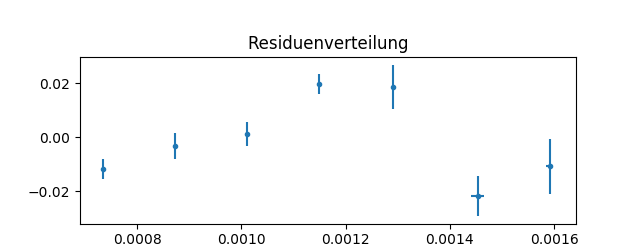
\includegraphics[width=0.6\linewidth]{residuen_laufzeit}
		\end{center}
		
	\end{frame}

	\begin{frame}
		\frametitle{Laufzeitmessung \qquad Auswertung II}
		\begin{itemize}
			\item Kalibration Poti: $k:=\frac{\Delta s}{\Delta R} =  (15,99 \pm 0,07) \frac{cm}{k\Omega}$\\ [0.5cm]
			%\item Laufzeitmessung: $\frac{\Delta R}{\Delta t} = (2181,55 \pm 22,77) \frac{k\Omega}{s}$
			
			
			\item Regression: $R(t)=a t+b$
			\item $a = \frac{\Delta R}{\Delta t} = 2181.54 k\Omega/s \quad \sigma_a=22.77 k\Omega/s$
			\item $b=-1.08 k\Omega \quad \sigma_b=0.03 k\Omega$
			\item $\chi^2/ndof=2.08$
			\item $v=\frac{\Delta s}{\Delta t} = k\cdot a = 348,90 m/s$
			\item $\Rightarrow \sigma_{v,stat.}=3,64m/s$
			\item $\Rightarrow \sigma_{v,syst.}=1,53m/s$ \\ [0.4cm]
			\item Theoriewert: $v = 345,14 m/s$
			
		\end{itemize}
		
		%$\Rightarrow v = \frac{\Delta s}{\Delta t} = (348,90 \pm 3,64 \pm 1,53) \frac{m}{s}$ \\ [0.3cm]
	%\qquad $\sigma _{stat} = v \frac{\sigma _{\Delta R/\Delta t}}{\Delta R / \Delta t}$ \qquad $\sigma _{sys} = v \frac{\sigma _{\Delta s/\Delta R}}{\Delta s / \Delta R}$
	\end{frame}
	
	
	
	
	
	
	
	
	
	\begin{frame}{Resonanzfrequenzen - Aufbau}
	\begin{figure}
	\begin{flushleft}
	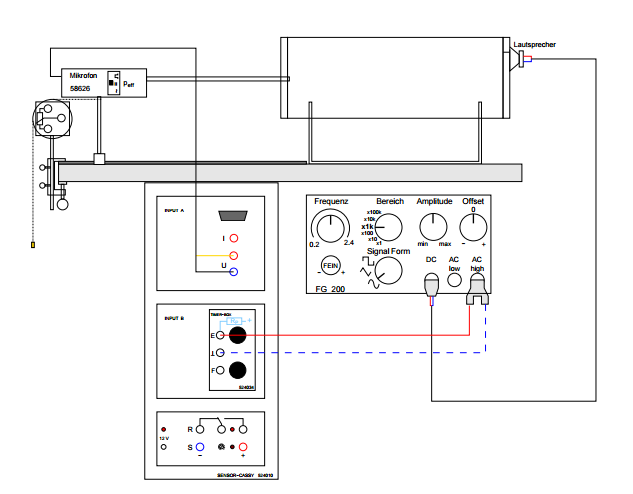
\includegraphics[scale=0.35]{aufbau}
	\end{flushleft}
	\end{figure}
	
	\begin{flushright}
	\begin{itemize}
	\item  Messbereich Spannung: $0-3V$ ,Nullpunkt links, gemittelt über $1s$.
	\item Timer-Box Bereich bis $5000Hz$, Torzeit $1s$
	\item manuelle Messung
	\end{itemize}
	\end{flushright}
	\end{frame}
	
	\begin{frame}{Resonanzfrequenzen - Ergebnisse I}
	\begin{figure}
	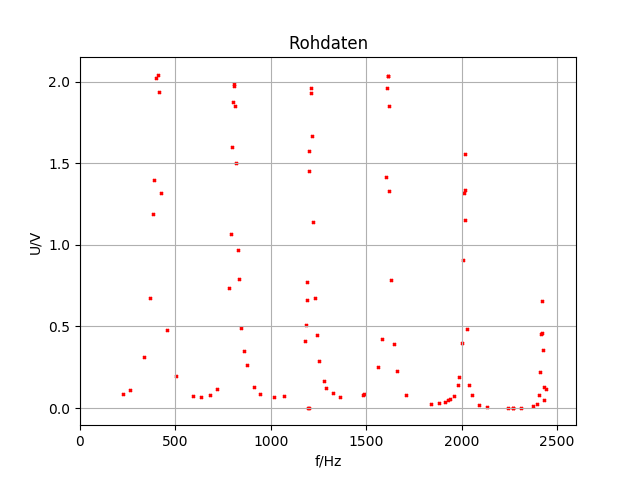
\includegraphics[scale=0.5]{rohres}
	\end{figure}
	\end{frame}
	
	\begin{frame}{Resonanzfrequenzen - Ergebnisse II}
	\begin{table}
	\begin{tabular}{|c|c|c|}
	\hline 
	$n$ & $f[Hz]$ & $\sigma_f$ \\ 
	\hline 
	1 & 404.11 & 1.47 \\ 
	\hline 
	2 & 809.60 & 1.72 \\ 
	\hline 
	3 & 1209.22 & 1.29 \\ 
	\hline 
	4 & 1613.86 & 1.32 \\ 
	\hline 
	5 & 2013.32 & 1.29 \\ 
	\hline 
	6 & 2420.10 & 0.96 \\ 
	\hline
	\end{tabular} 
	\end{table}
	\end{frame}
	
	\begin{frame}{Resonanzfrequenzen - Auswertung I}
	\begin{figure}
	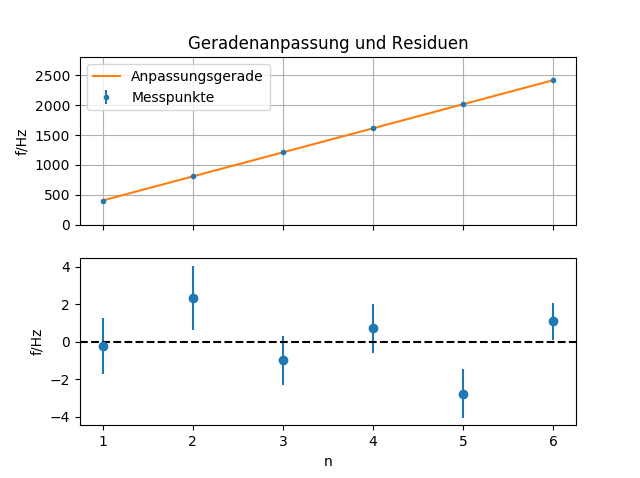
\includegraphics[width=\linewidth , height=0.75\textheight]{fitplot}
	\end{figure}
	\end{frame}
	
	\begin{frame}{Resonanzfrequenzen - Auswertung II}
	\begin{itemize}
	\item Regression: $f(n)=a n+b$
	\item $a=402.94Hz \quad \sigma_a=0.30Hz$
	\item $b=1.40Hz \quad \sigma_b=1.32Hz$
	\item $\chi^2/ndof=2.13$
	\item $v= 2*a*L = 344.91m/s$
	\item $\Rightarrow \sigma_{v,stat.}=0.35m/s$
	\item $\Rightarrow \sigma_{v,syst.}=0.56m/s$ \\ [0,4cm]
	\item Theoriewert: $v=346,23 m/s$
	\end{itemize}
	\end{frame}
	
	\begin{frame}{Druckverlauf - Aufbau}
	\begin{itemize}
	\item Aufbau weitestgehend identisch zu Teilv. 1
	\item $f=2017Hz$
	\item Messbereich Spannung $0-3V$, Nullpunkt links und gemittelt über $100ms$.
	\item Widerstandsbereich $0-3k \Omega$
	\item Messparameter automatisch $100ms$.
	\end{itemize}
	
	\end{frame}
	
	\begin{frame}{Druckverlauf - Ergebnisse}
	\begin{figure}
	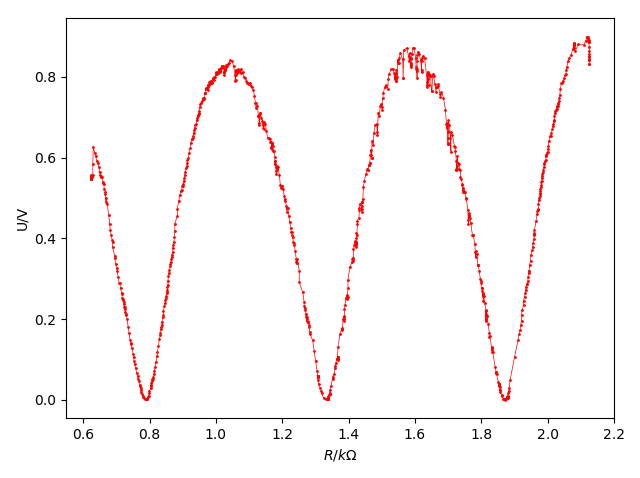
\includegraphics[scale=0.5]{druckverlauf}
	\end{figure}
	\end{frame}
	
	\begin{frame}{Ergebnisse und Auswertung}
	\begin{table}
	\begin{tabular}{|c|c|c|}
	\hline 
	n & $R[k\Omega]$ & $\sigma_R[k\Omega]$ \\ 
	\hline 
	1 & 0.788 & 0.006 \\ 
	\hline 
	2 & 1.344 & 0.006 \\ 
	\hline 
	3 & 1.872 & 0.006 \\ 
	\hline 
	\end{tabular} 
	\end{table}
	
	\begin{figure}
	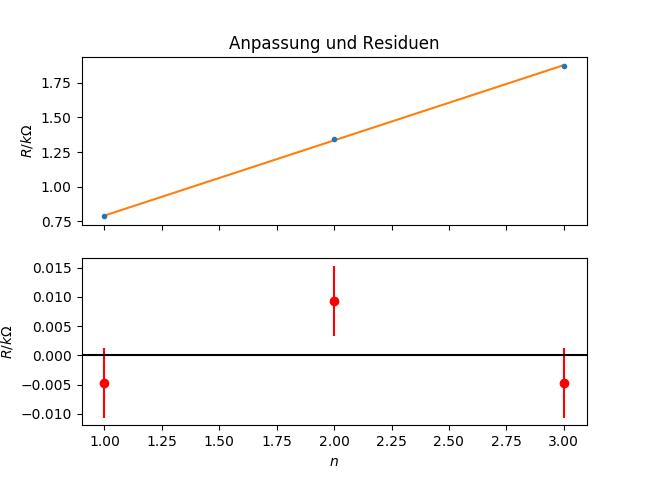
\includegraphics[scale=0.37]{fitdruckknoten}
	\end{figure}
	\end{frame}
	
	\begin{frame}
	\begin{itemize}
	\item $R(n)=a \cdot n+b$
	\item $a=0.542k\Omega \quad \sigma_{a}=0.004k\Omega$
	\item $b=0.251k\Omega \quad \sigma_b=0.009k\Omega$
	\item $\chi^2/ndof=3.630$
	\item $\lambda=2Ka=17.31cm$
	\item $f=2017.0Hz \quad \Rightarrow \quad v=\lambda f = 349.14m/s$
	\item $\sigma_f=0.3Hz \quad \Rightarrow \sigma_{v,stat.}=2.63m/s$
	\item $\sigma_{v,syst.}=f \sigma_{\lambda,syst.}=1.61m/s$ \\ [0,4cm]
	\item Theoriewert: $v=346,23 m/s$
	\end{itemize}
	\end{frame}
	
	
	
	
	
	
	
	
	
	
\begin{frame}{Schall in Festkörpern: Grundlagen}
	\begin{itemize}
		\item Ziel: Bestimmung der Schallgeschwindigkeit und des Elastizitätsmoduls in Metallen
		\item Schallgeschwindigkeit:
		\begin{equation}
		v_l = \lambda_0 \cdot f_0 = 2 \cdot L \cdot f_0
		\label{eq:002}
		\end{equation}
		\item Elastizitätsmodul:
		\begin{equation}
		E = \rho \cdot v_L^2 =  16 f_0^2 \cdot \dfrac{L M}{\pi D^2}.
		\label{eq:003}
		\end{equation}
	\end{itemize}
\end{frame}

\begin{frame}{Aufbau}
	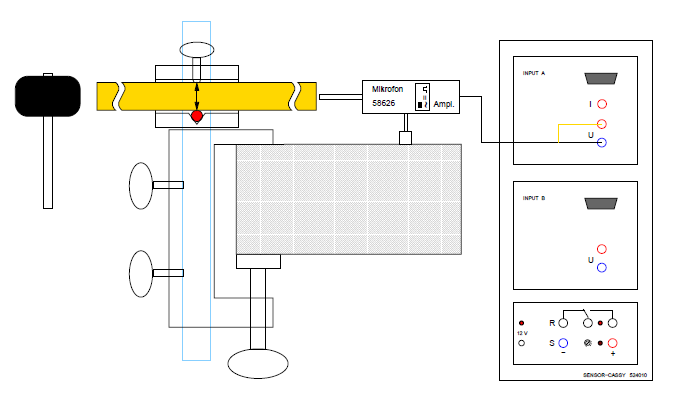
\includegraphics[width=\linewidth,height=\textheight,keepaspectratio]{Bilder/AufbauMessungSchallgeschwindigkeitMetallstab.PNG}
	\centering
\end{frame}

\begin{frame}{Schall in Festkörpern: Durchführung}
	\begin{itemize}
		\item Mikrofon im Amplitudenmodus
		\item CASSY-Eistellungen
		\begin{itemize}
			\item kleines Abtastinervall($50\mu s$)
			\item 16000 Messungen
			\item mittlerer Messbereich($-3V\leq U\leq 3V$)
		\end{itemize}
		\item Messwerte
		\begin{itemize}
			\item Länge: Einfachmessung mit $\sigma_{stat}\approx0.3mm$ und $\sigma_{sys}=0.56mm$
			\item Durchmesser, Masse, Frequenz werden durch Mehrfachmessung bestimmt
		\end{itemize}
		\item Schlag auf Metallstab möglichst eben auf Stabende
		\item Messung wird kurze Zeit nach Anschlag gestartet
	\end{itemize}
\end{frame}

\begin{frame}{Schall in Festkörpern: Ergebnisse}
	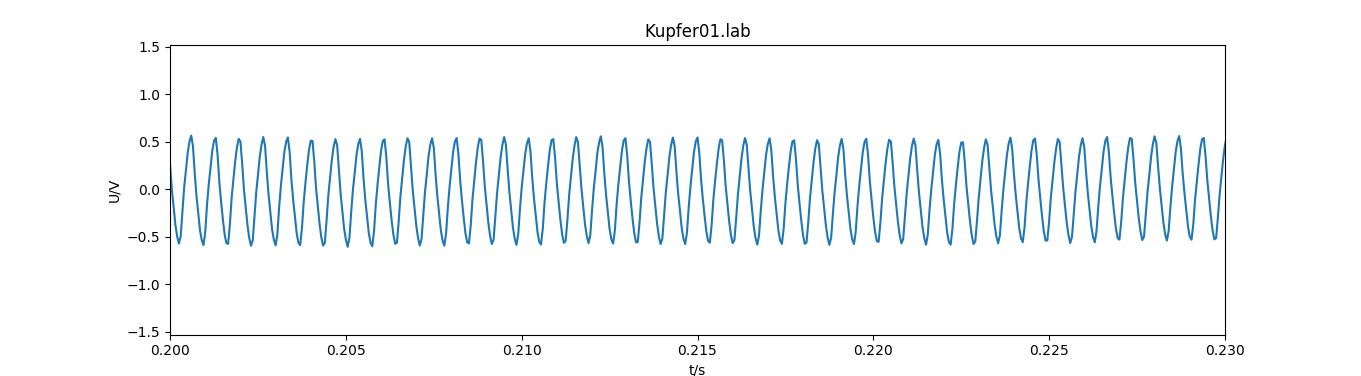
\includegraphics[width=\linewidth,height=\textheight,keepaspectratio]{Bilder/Kupfer01.PNG}
	\begin{itemize}
		\item Auswertung der Messergebnisse durch eine Fast-Fourier-Transformation
	\end{itemize}
\end{frame}

\begin{frame}{Schall in Festkörpern: Fourieranalysen}
	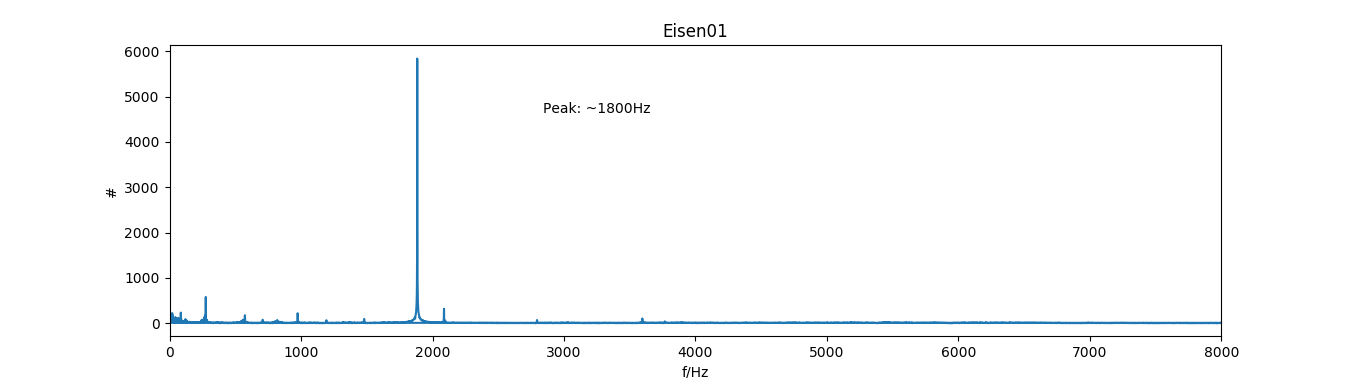
\includegraphics[width=0.5\textwidth, height=0.4\textheight]{Bilder/Eisen01_fourier.png}
	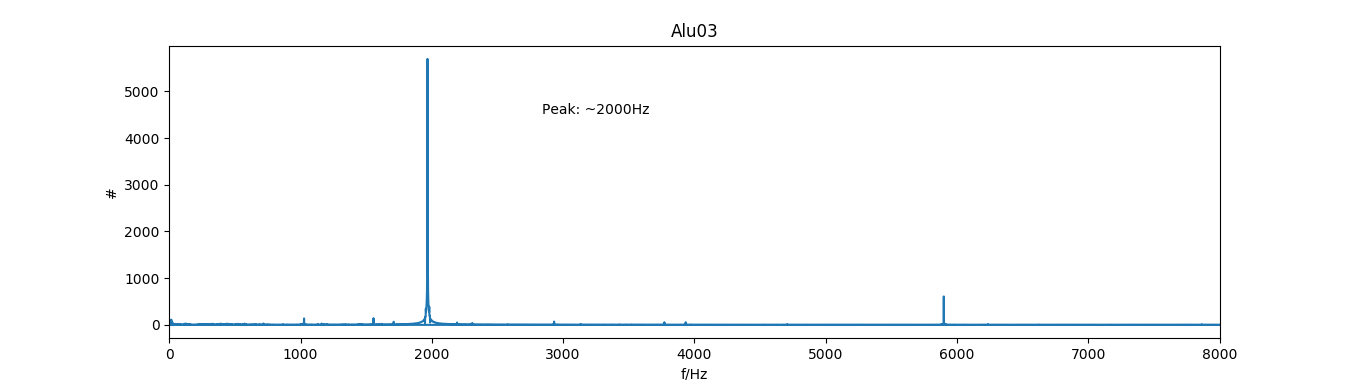
\includegraphics[width=0.5\linewidth,height=0.4\textheight]{Bilder/Alu03_fourier.png}\\
	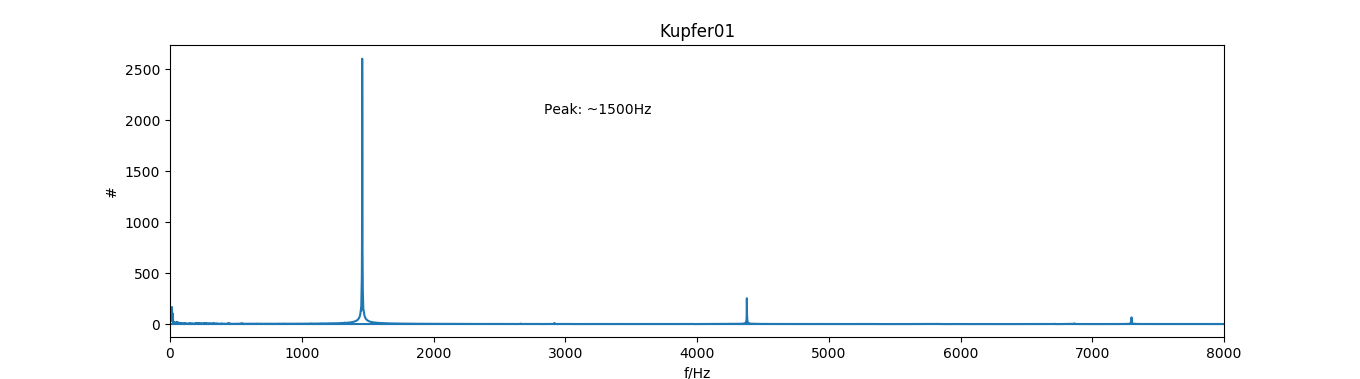
\includegraphics[width=0.5\linewidth,height=0.4\textheight]{Bilder/Kupfer01_fourier.png}
	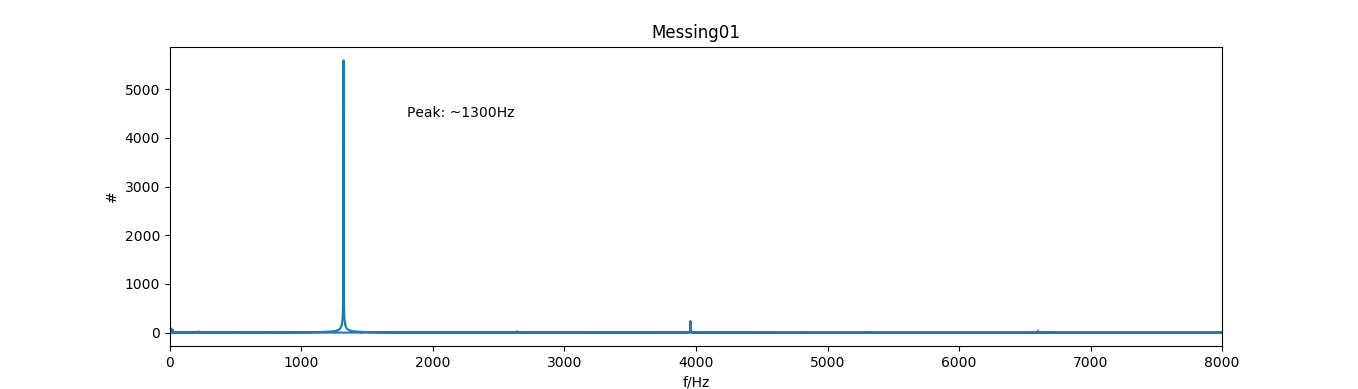
\includegraphics[width=0.5\linewidth,height=0.4\textheight]{Bilder/Messing01_fourier.png}\\
\end{frame}

\begin{frame}{Schall in Festkörpern: Messergebnisse}
	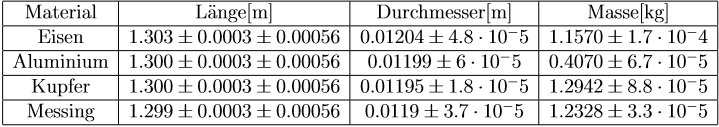
\includegraphics[width=\linewidth,height=\textheight,keepaspectratio]{Bilder/Material_Metalle.PNG}\\
	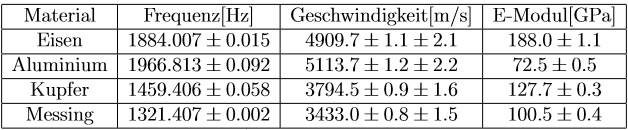
\includegraphics[width=\linewidth,height=\textheight,keepaspectratio]{Bilder/Ergebnisse_Metall.PNG}\\
	
\end{frame}

\begin{frame}{Schall in Festkörpern: Literaturwerte}
	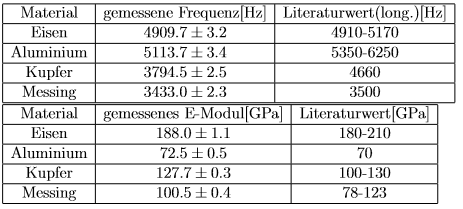
\includegraphics[width=\linewidth,height=\textheight,keepaspectratio]{Bilder/Literaturwerte_Metalle.PNG}\\
	\begin{itemize}
		\item Fazit:
		\begin{itemize}
			\item Ergebnisse sind sinnvoll
			\item Abweichungen durch ungenaue Materialeigenschaften
		\end{itemize}
	\end{itemize}
\end{frame}








\begin{frame}{Akustik der Gitarre Teil 1: Grundlagen}
	Ziel des Versuchs: Messung der Schwebung \\
	Superpositionsprinzip: $\sum_{n=1}^N A_n \cdot \sin(w_nt) \cdot \sin(kx)$ \\
	Hier:
	\[A(x=0, t) = A_0 \cdot \sin(w_st) \cdot \sin(w_{res}t)\]
	mit
	\[w_s = \dfrac{w_1 - w_2}{2} \quad und \quad w_{res} = \dfrac{w_1 + w_2}{2}\]
\end{frame}

\begin{frame}{Akustik der Gitarre Teil 1: Aufbau}
	\begin{figure}
		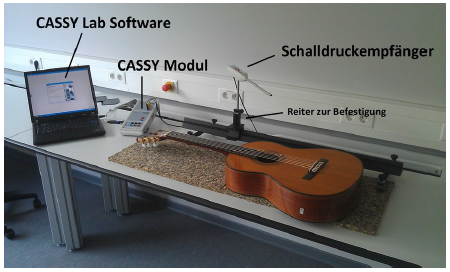
\includegraphics[scale=0.8]{Bilder/AufbauAkustikGitarre.PNG}
		\centering
	\end{figure}
\end{frame}

\begin{frame}{Akustik der Gitarre Teil 1: Durchführung}
	Messeinstellungen:
	\begin{itemize}
		\item Messbereich $|U| \leq 3V$
		\item Intervall $500 \mu s$
		\item Messzeit $8s$
	\end{itemize}
	Durchführung:
	\begin{itemize}
		\item Gitarre stimmen
		\item Eine Saite verstimmen
		\item Zwei Saiten anschlagen
		\item Messung verzögert starten
	\end{itemize}
\end{frame}

\begin{frame}{Akustik der Gitarre Teil 1: Rohdaten}
	\begin{figure}
		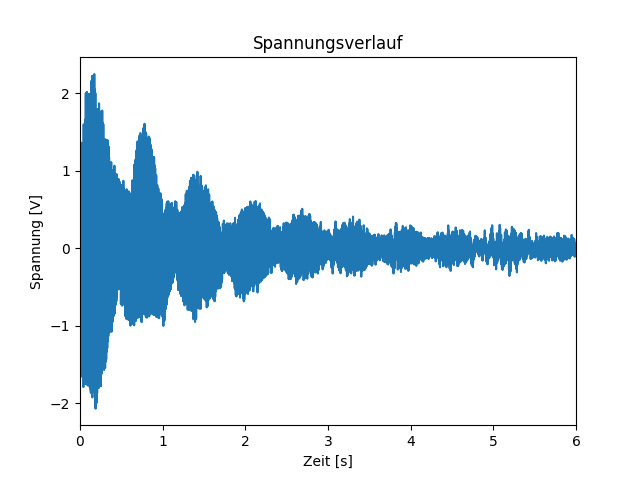
\includegraphics[scale=0.6]{Bilder/Schwebung_roh.png}
	\end{figure}
\end{frame}

\begin{frame}{Akustik der Gitarre Teil 1: Frequenzspektrum}
	\begin{figure}
		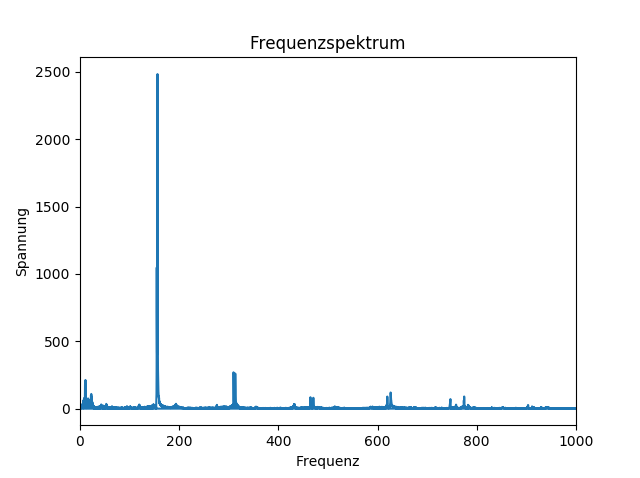
\includegraphics[scale=0.3]{Bilder/Frequenzspektrum_ges.png}
	\end{figure}
	\begin{figure}
		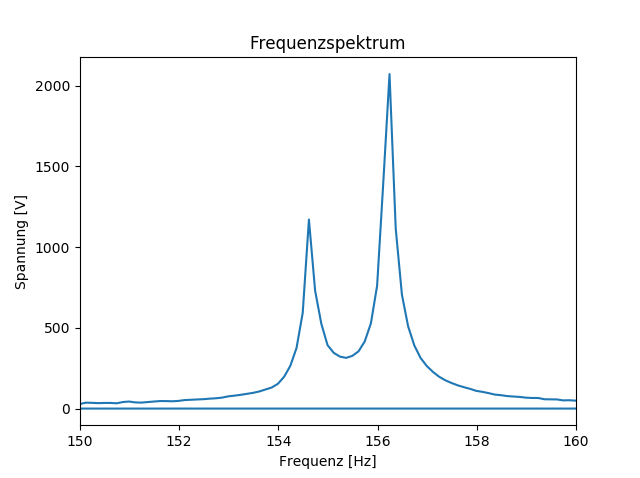
\includegraphics[scale=0.3]{Bilder/Frequenzspektrum_zoom.png}
	\end{figure}
\end{frame}

\begin{frame}{Akustik der Gitarre Teil 1: Auswertung}
	\begin{figure}
		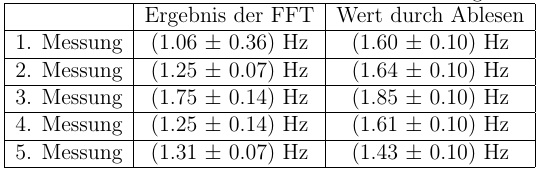
\includegraphics[scale=0.8]{Bilder/SchwebungErgebnisTabelle.PNG}
	\end{figure}
	Fazit: Fehler der FFT schwankt stark, \\ 
	Abgelesener Wert größer als  FFT
\end{frame}

\begin{frame}{Akustik der Gitarre Teil 2: Grundlagen}
	Ziel des Versuchs: Bestimmung von $\sqrt{\dfrac{T}{\mu}}$ \\
	\[f_n = \dfrac{n}{2L} \cdot \sqrt{\dfrac{T}{\mu}}\]
	Grundschwingung für $n = 1$
\end{frame}

\begin{frame}{Akustik der Gitarre Teil 2: Aufbau}
	\begin{figure}
		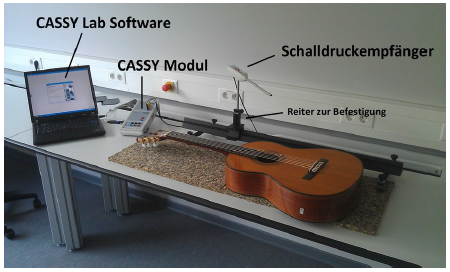
\includegraphics[scale=0.8]{Bilder/AufbauAkustikGitarre.PNG}
		\centering
	\end{figure}
\end{frame}

\begin{frame}{Akustik der Gitarre Teil 2: Durchführung}
	Messeinstellungen:
	\begin{itemize}
		\item Messbereich $|U| \leq 3V$
		\item Intervall $200 \mu s$
		\item Messzeit $3,2s$
	\end{itemize}
	Durchführung:
	\begin{itemize}
		\item Gitarre stimmen (Frequenz messen mit CASSY)
		\item Gitarre vermessen
		\item Saite verkürzen und anschlagen
		\item Messung verzögert starten
	\end{itemize}
\end{frame}

\begin{frame}{Akustik der Gitarre Teil 2: Rohdaten}
	\begin{figure}
		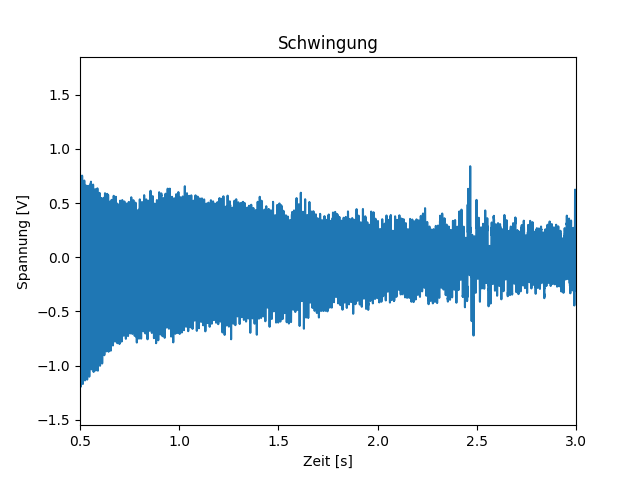
\includegraphics[scale=0.6]{Bilder/Gitarre_Schwingung.PNG}
	\end{figure}
\end{frame}

\begin{frame}{Akustik der Gitarre Teil 2: Frequenzspektrum}
	\begin{figure}
		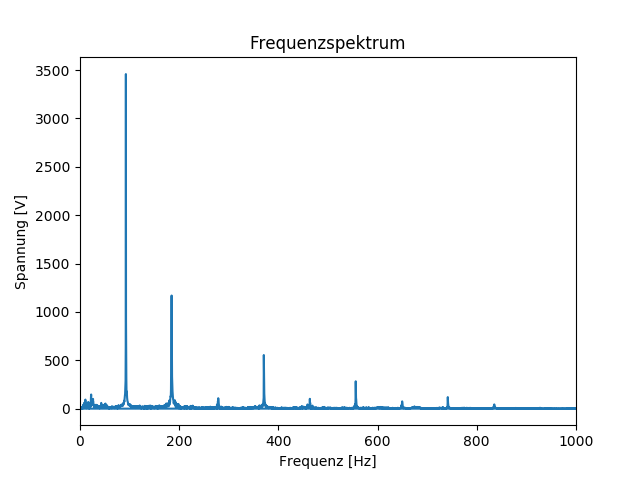
\includegraphics[scale=0.6]{Bilder/FrequenzspektrumGitarrensaite.PNG}
	\end{figure}
\end{frame}

\begin{frame}{Akustik der Gitarre Teil 2: Auswertung}
	\begin{figure}
		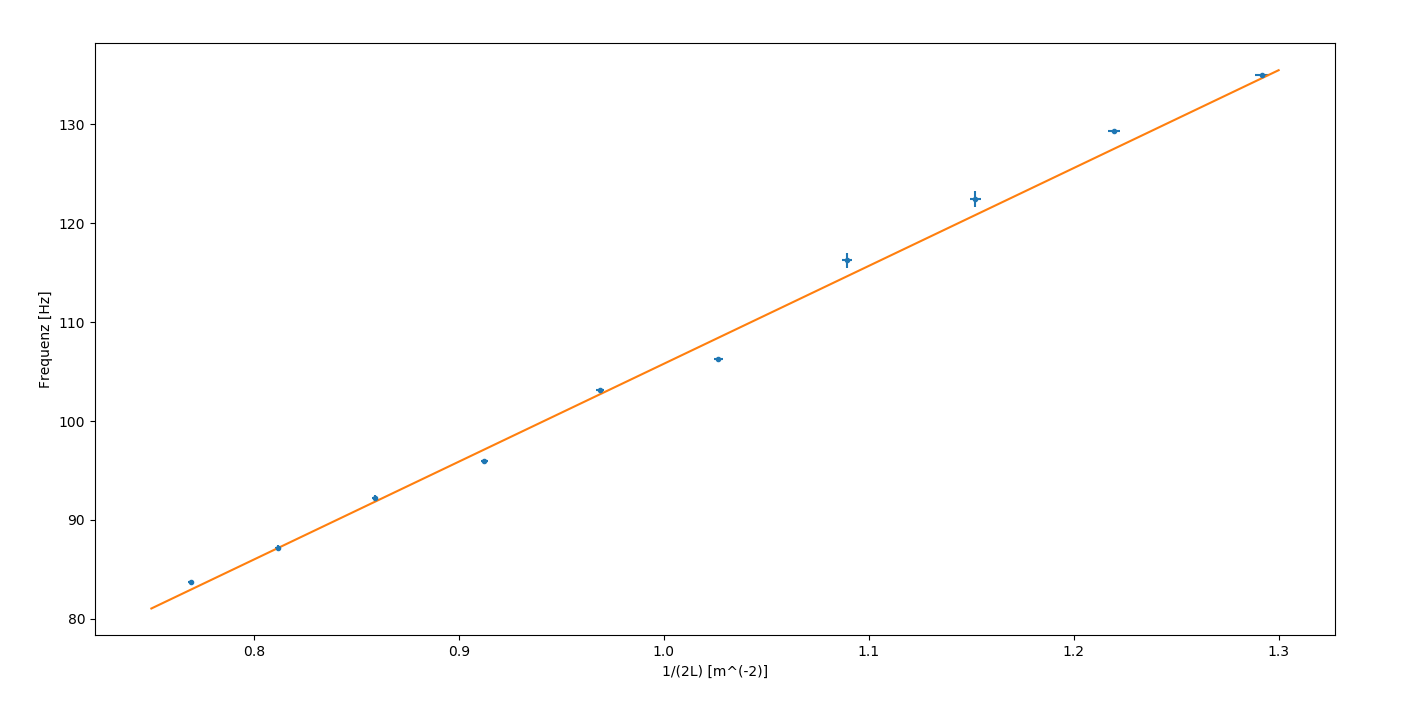
\includegraphics[scale=0.3]{Bilder/SpannungMassebelagLineareRegression.PNG}
	\end{figure}
\end{frame}

\begin{frame}{Akustik der Gitarre Teil 2: Auswertung}
	Lineare Regression
	\[\sqrt{\dfrac{T}{\mu}} = (98,98 \pm 2,67)\sqrt{\dfrac{Nm}{kg}}\]
	Mit $T = 63,50N$ und $\mu = 5,67 \cdot 10^{-3} \dfrac{kg}{m}$
	\[\sqrt{\dfrac{T}{\mu}} = 105,82 \sqrt{\dfrac{Nm}{kg}}\]
	Fazit: Vorgehensweise ist gute Möglichkeit $\sqrt{\dfrac{T}{\mu}}$ zu bestimmen
\end{frame}





	
\end{document}